\chapter{Results}

\section{Computational results}


\subsection{Runge-Kutta Solver Accuracy}

\begin{figure}[bth]
	\myfloatalign
	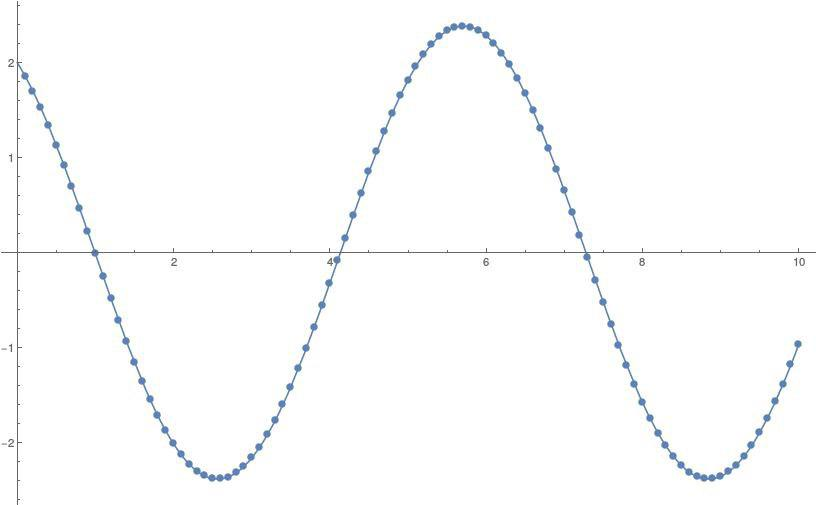
\includegraphics[width=.8\linewidth]{gfx/stepcomputation}
	\caption[Automatic step computation]{Automatic step computation}
	\label{fig:stepsize}
\end{figure}

\begin{figure}[bth]
	\myfloatalign
	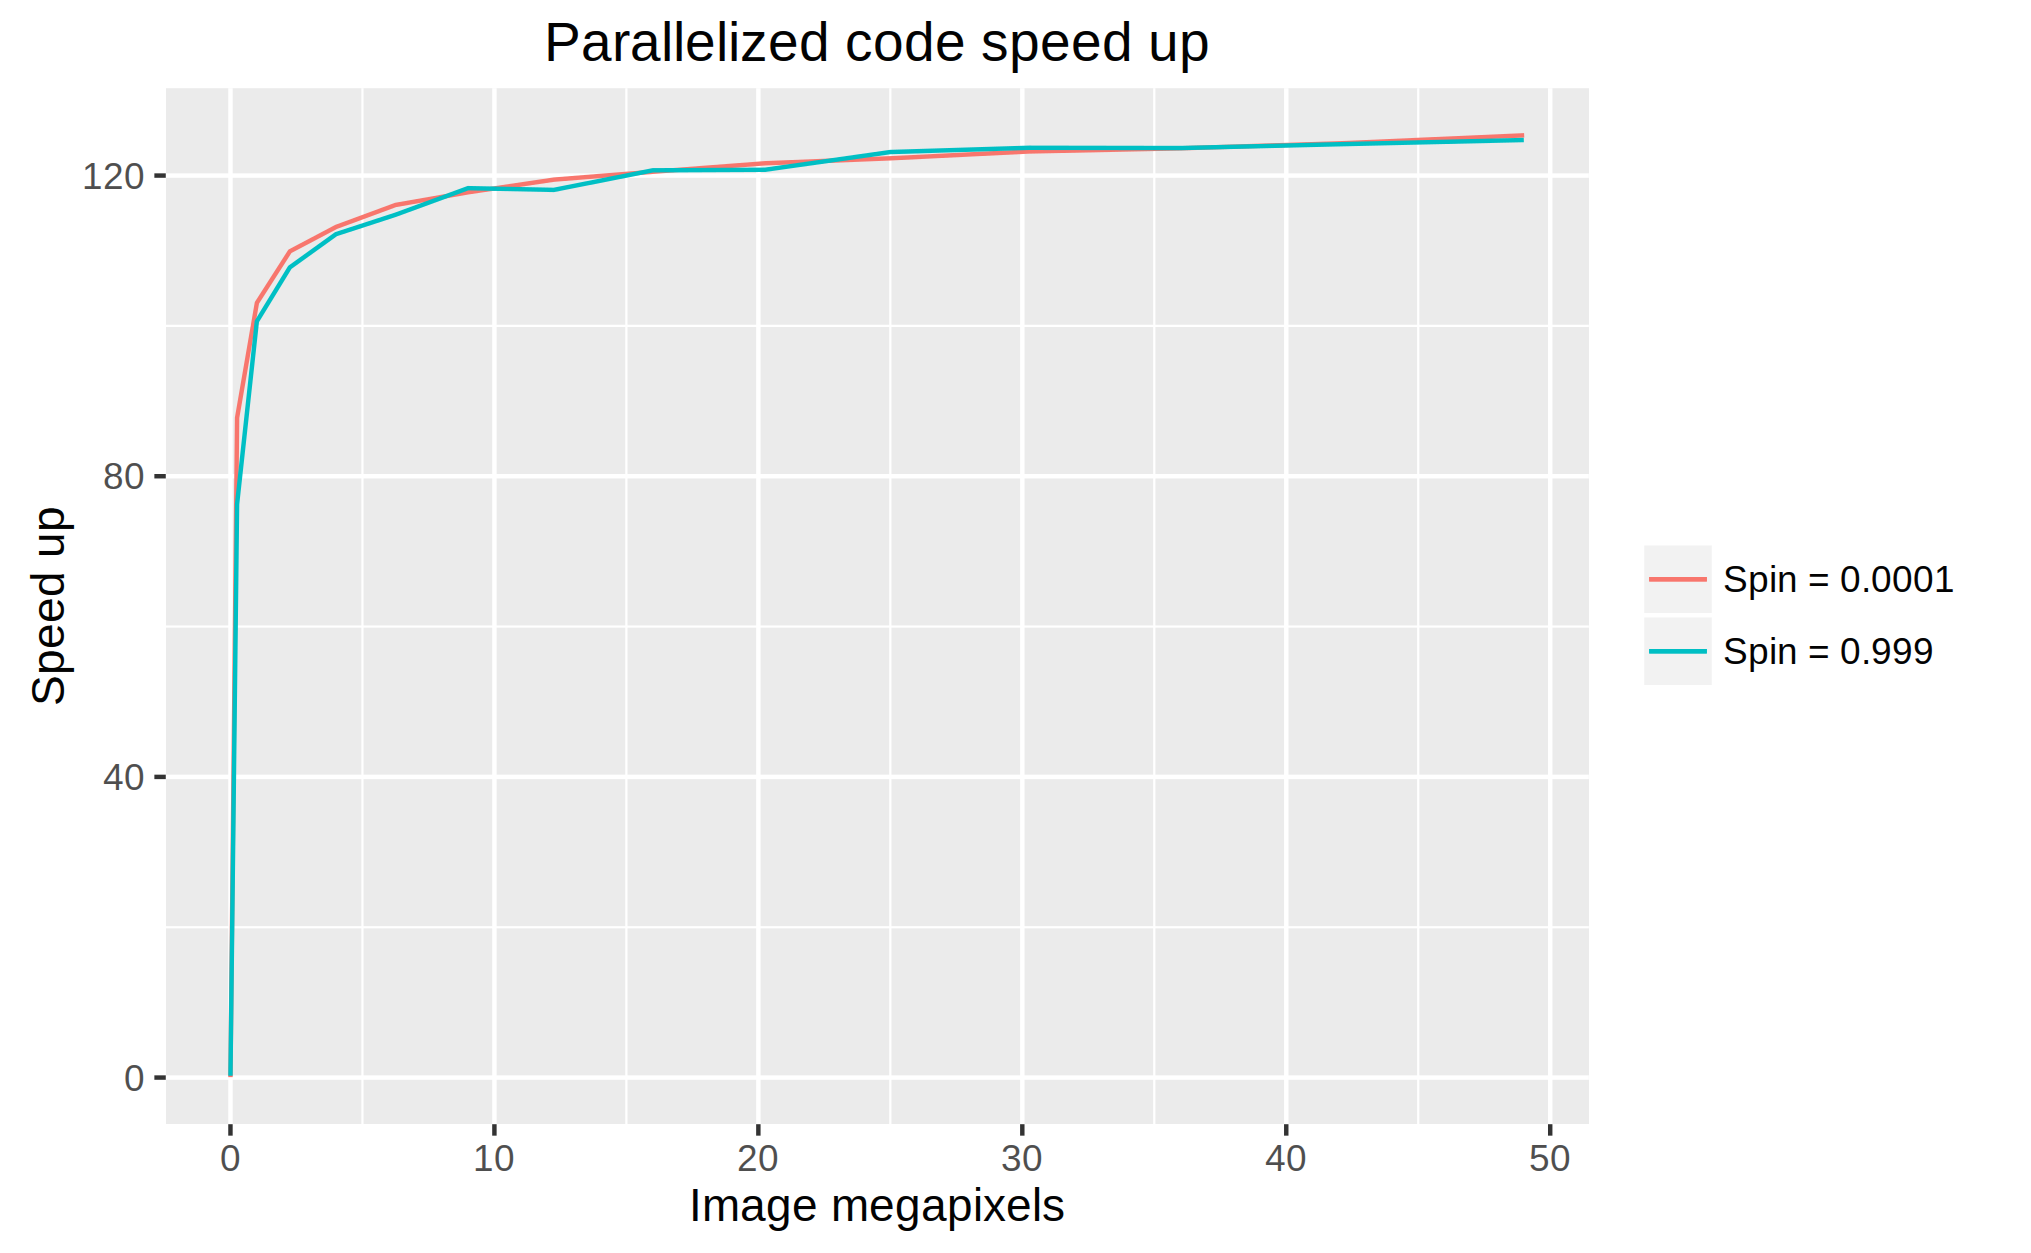
\includegraphics[width=.8\linewidth]{gfx/speedup}
	\caption[Speed up with different spins]{Speed up with different spins}
	\label{fig:speedup}
\end{figure}

\begin{figure}[bth]
	\myfloatalign
	{\label{fig:example-b}%
		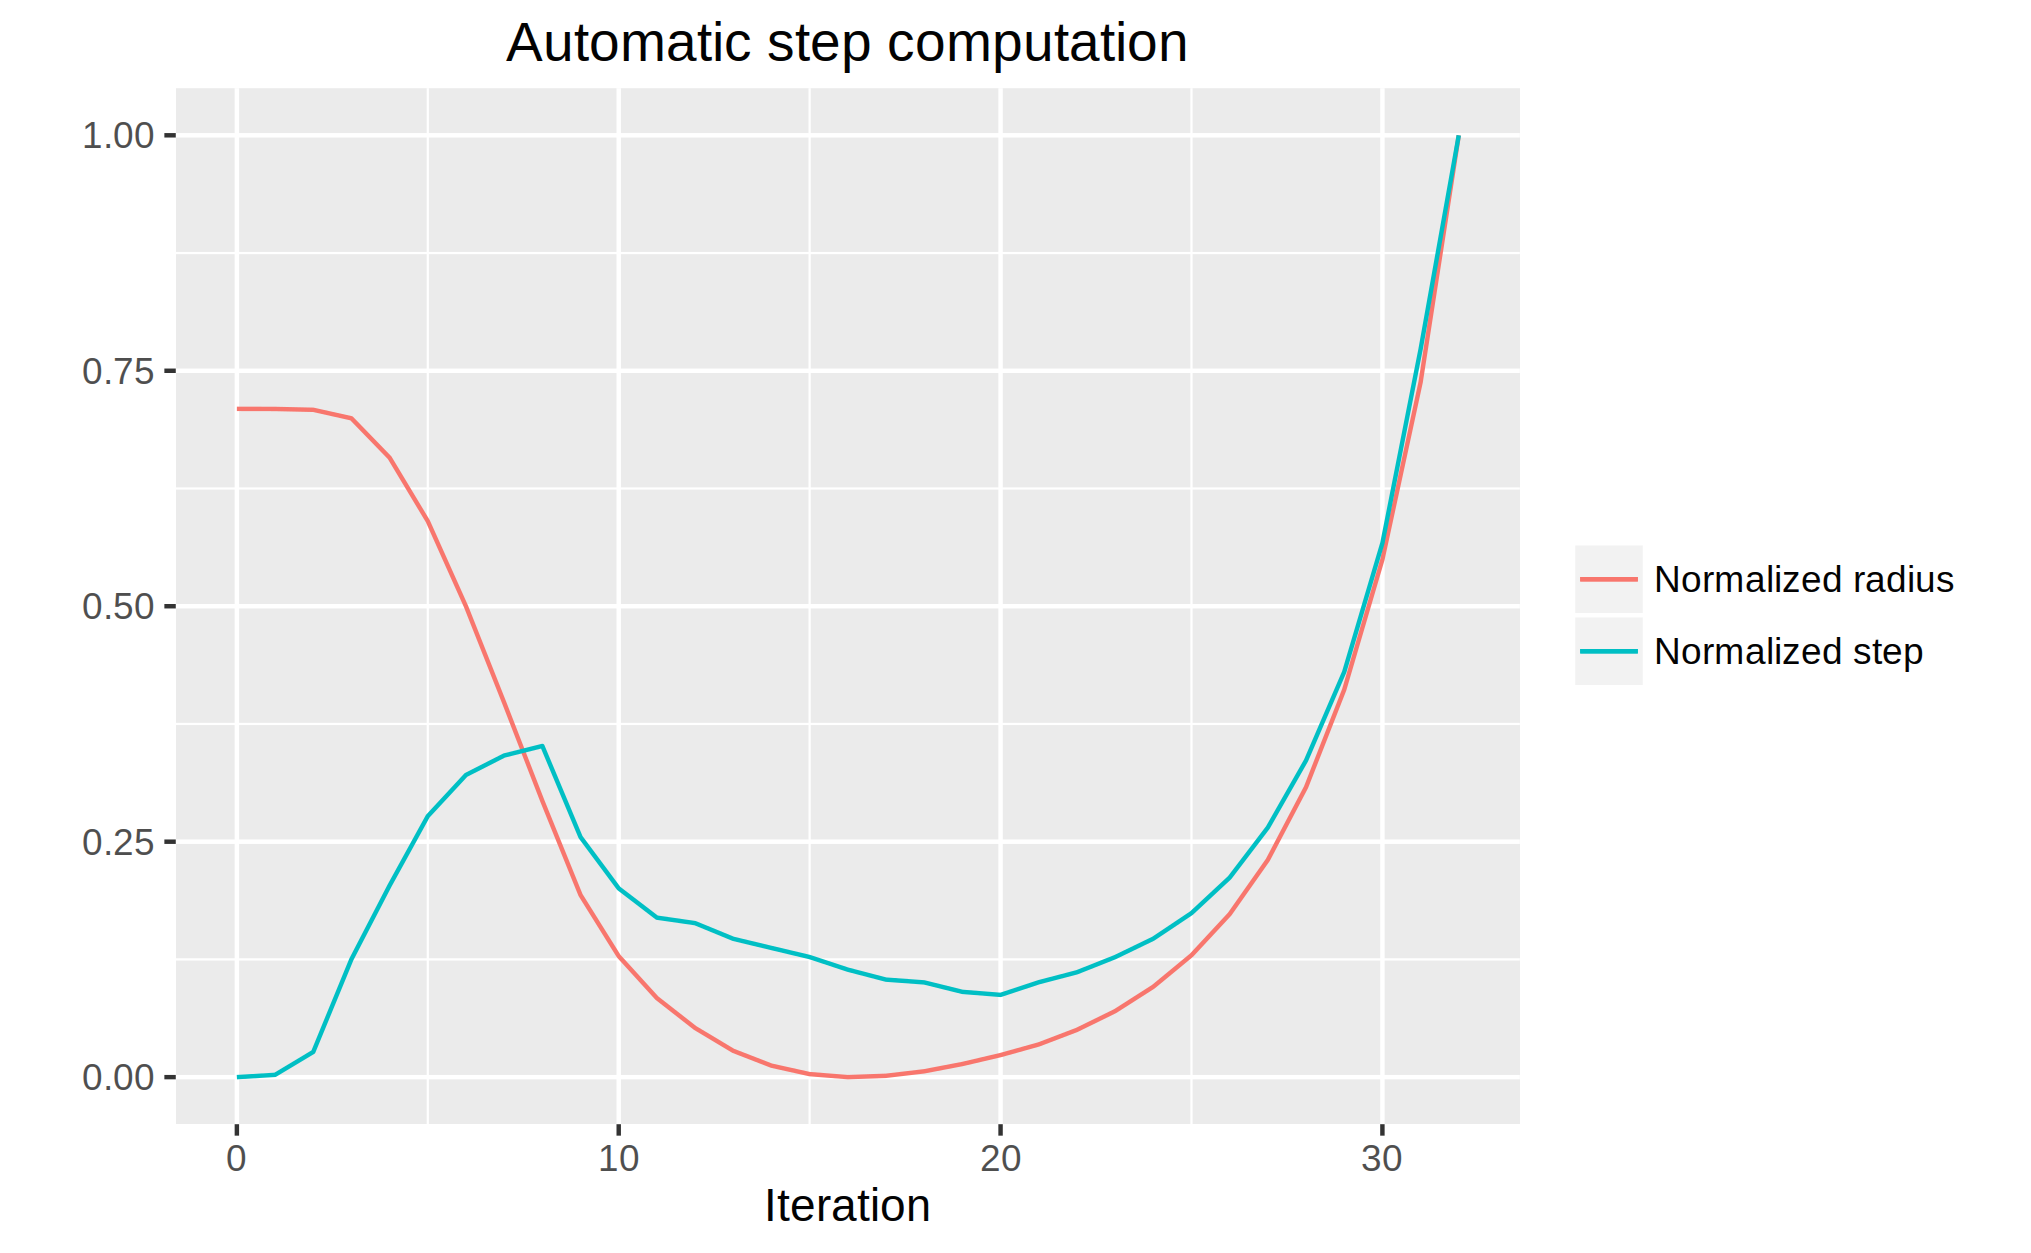
\includegraphics[width=.8\linewidth]{gfx/stepradius1}} \\
	{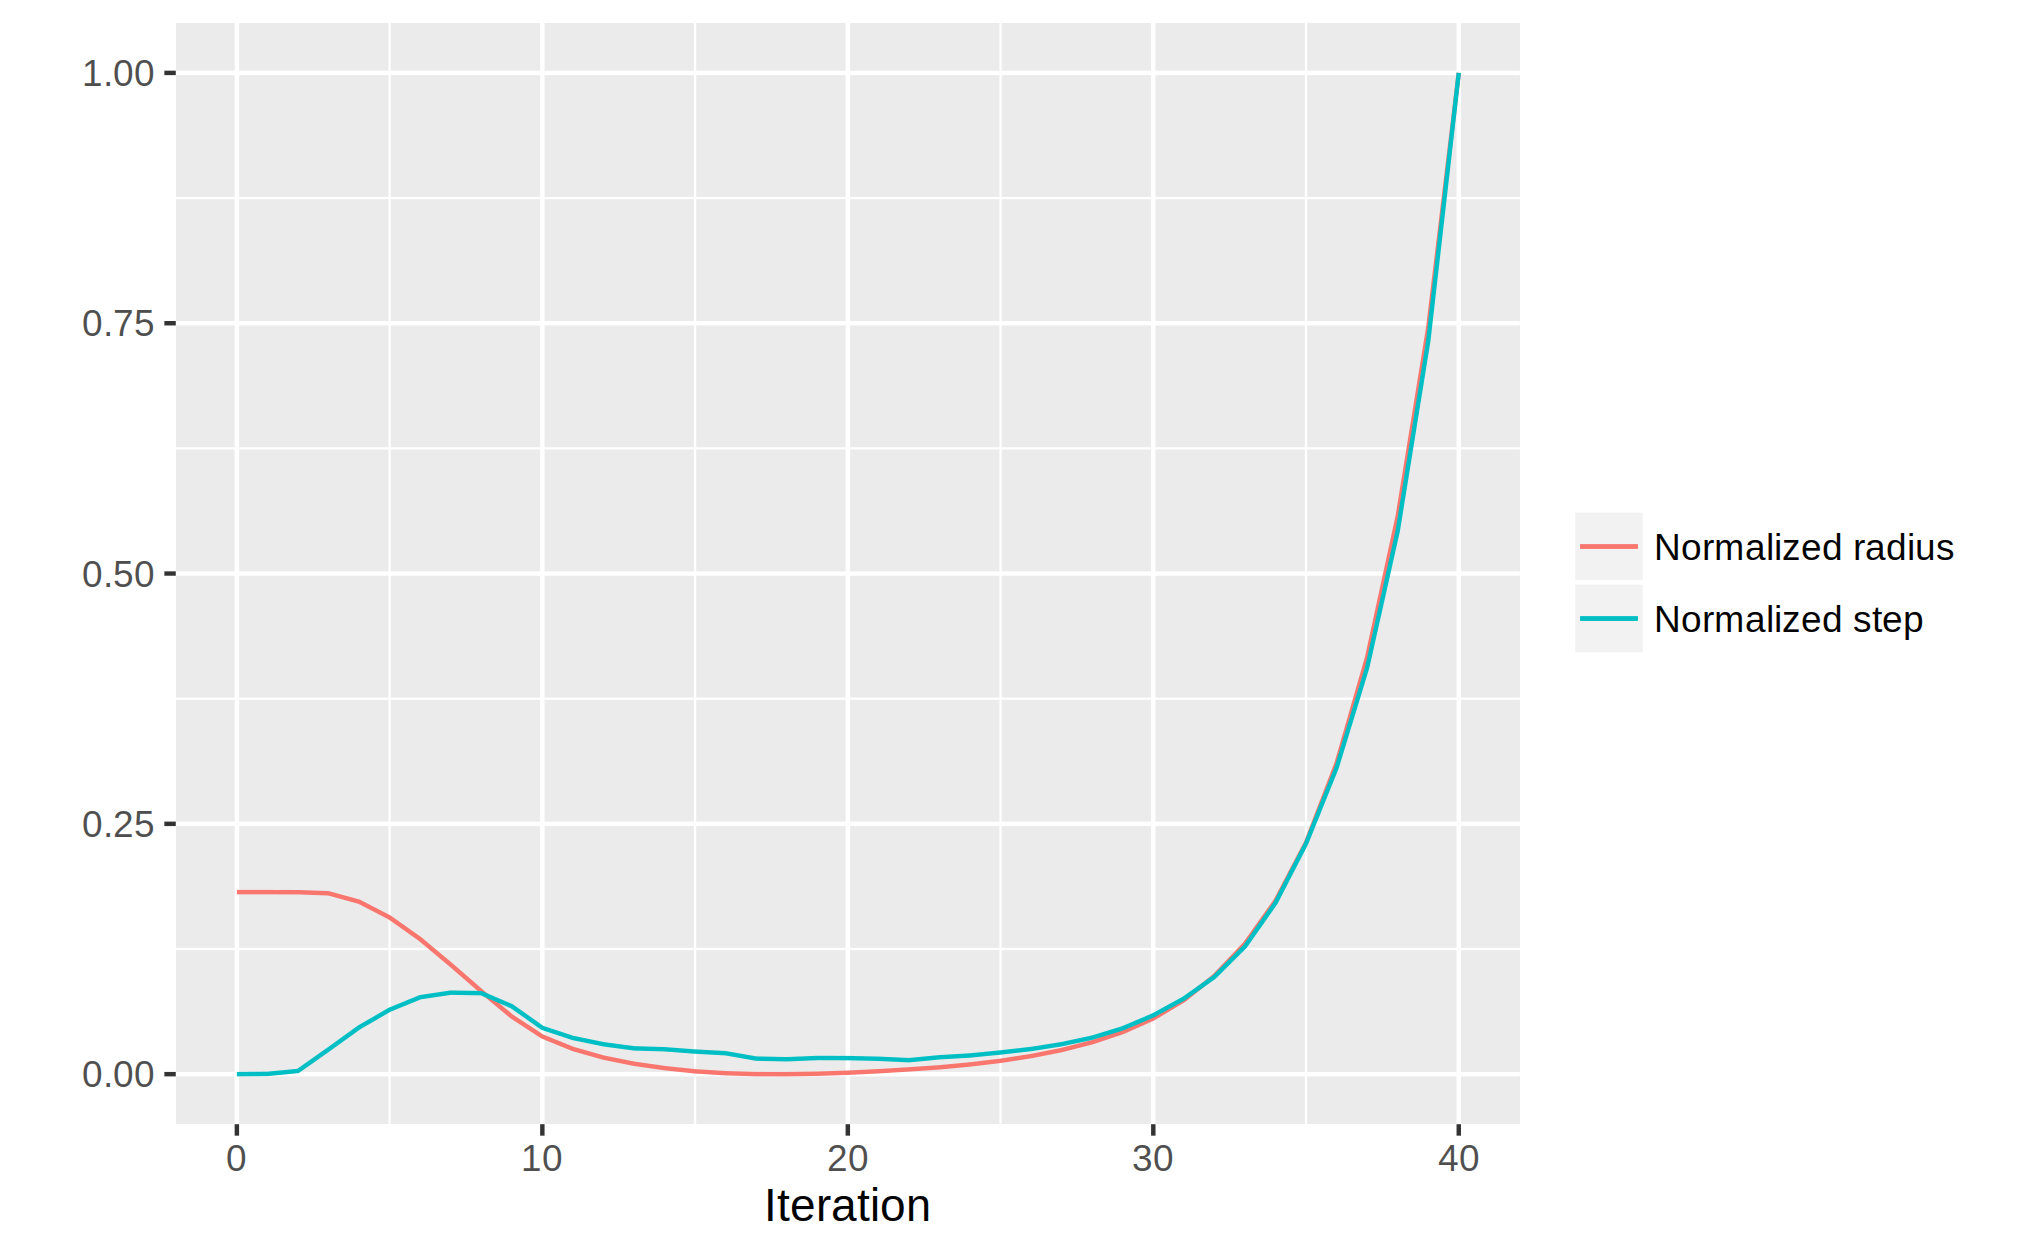
\includegraphics[width=.8\linewidth]{gfx/stepradius2}}
	\caption[Step size and radius comparison]{Step size and radius comparison}\label{fig:step}
\end{figure}


\section{Scientific results}